\section{Graph Based Problem Formulation}
A solution to the bus charge problem must reveal both \textit{when} and \textit{to which} bus a charger should connect. This suggests an approach with two dimensions, the first characterizing time and the second encoding charger connections as charge-states. This 2-D representation is encoded as a grid where time is given discretely in a left to right fashion and charge-states extend vertically as seen in figure \ref{fig:graphGridStructure}. In an effort to accurately represent charger use, the available charge-states include `connected' states for each bus and a `disconnected' state for idle periods. The intersection of charge-states and time indices is represented by a node, denoted $n_{i,j}$ which represents charge-state $i$ at time $t_j$ (see figure \ref{fig:graphGridStructure}).  
\par A complete grid, however, implies that chargers can always connect to all buses.  This is not always the case as a bus's schedule is divided into `on-route' and `in-station' segments. While on-route, buses depart to provide transit services and are unable to charge. To reflect this constraint, nodes are also used to denote availability and are removed when a bus is on-route (see figure \ref{fig:busAvailEncode}). 

\begin{figure*}
	\subfloat[Graph showing buses and timesteps \label{fig:graphGridStructure}]{
		\centering
		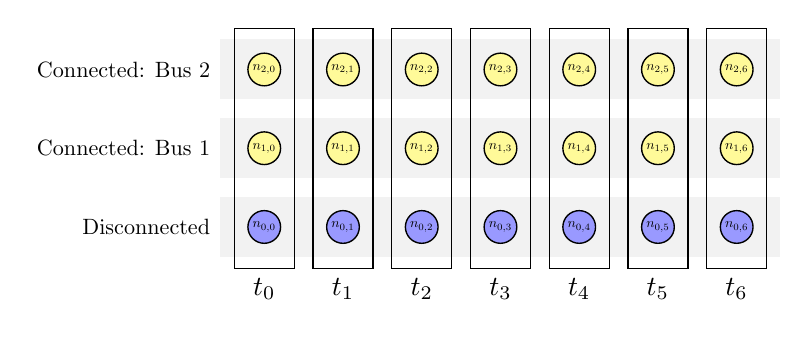
\begin{tikzpicture}
			\node[rectangle, fill=gray!10, minimum width=2.8in, minimum height=.3in,label=left:\scalebox{0.8}{Connected: Bus 2}](bus2Box) at (3,1){};
			\node[rectangle, fill=gray!10, minimum width=2.8in, minimum height=.3in,label=left:\scalebox{0.8}{Connected: Bus 1}](bus1Box) at (3,0){};
			\node[rectangle, fill=gray!10, minimum width=2.8in, minimum height=.3in,label=left:\scalebox{0.8}{Disconnected}](bus1Box) at (3,-1){};

			\node[circle, fill=yellow!40, line width=0.5pt, draw=black, minimum size=0.15in, inner sep=1pt](one) at (0,0){\scalebox{0.5}{$n_{1,0}$}};
			\node[circle, fill=yellow!40, line width=0.5pt, draw=black, minimum size=0.15in, inner sep=1pt](two) at (1,0){\scalebox{0.5}{$n_{1,1}$}}; 
			\node[circle, fill=yellow!40, line width=0.5pt, draw=black, minimum size=0.15in, inner sep=1pt](three) at (2,0){\scalebox{0.5}{$n_{1,2}$}};
			\node[circle, fill=yellow!40, line width=0.5pt, draw=black, minimum size=0.15in, inner sep=1pt](four) at (3,0){\scalebox{0.5}{$n_{1,3}$}};
			\node[circle, fill=yellow!40, line width=0.5pt, draw=black, minimum size=0.15in, inner sep=1pt](five) at (4,0){\scalebox{0.5}{$n_{1,4}$}};
			\node[circle, fill=yellow!40, line width=0.5pt, draw=black, minimum size=0.15in, inner sep=1pt](six) at (5,0){\scalebox{0.5}{$n_{1,5}$}};
			\node[circle, fill=yellow!40, line width=0.5pt, draw=black, minimum size=0.15in, inner sep=1pt](seven) at (6,0){\scalebox{0.5}{$n_{1,6}$}};

			\node[circle, fill=yellow!40, line width=0.5pt, draw=black, minimum size=0.15in, inner sep=1pt](eight) at (0,1){\scalebox{0.5}{$n_{2,0}$}};
			\node[circle, fill=yellow!40, line width=0.5pt, draw=black, minimum size=0.15in, inner sep=1pt](nine) at (1,1){\scalebox{0.5}{$n_{2,1}$}}; 
			\node[circle, fill=yellow!40, line width=0.5pt, draw=black, minimum size=0.15in, inner sep=1pt](ten) at (2,1){\scalebox{0.5}{$n_{2,2}$}};
			\node[circle, fill=yellow!40, line width=0.5pt, draw=black, minimum size=0.15in, inner sep=1pt](eleven) at (3,1){\scalebox{0.5}{$n_{2,3}$}};
			\node[circle, fill=yellow!40, line width=0.5pt, draw=black, minimum size=0.15in, inner sep=1pt](twelve) at (4,1){\scalebox{0.5}{$n_{2,4}$}};
			\node[circle, fill=yellow!40, line width=0.5pt, draw=black, minimum size=0.15in, inner sep=1pt](thirteen) at (5,1){\scalebox{0.5}{$n_{2,5}$}};
			\node[circle, fill=yellow!40, line width=0.5pt, draw=black, minimum size=0.15in, inner sep=1pt](fourteen) at (6,1){\scalebox{0.5}{$n_{2,6}$}};

			\node[circle, fill=blue!40, line width=0.5pt, draw=black, minimum size=0.15in, inner sep=1pt](eight) at (0,-1){\scalebox{0.5}{$n_{0,0}$}};
			\node[circle, fill=blue!40, line width=0.5pt, draw=black, minimum size=0.15in, inner sep=1pt](nine) at (1,-1){\scalebox{0.5}{$n_{0,1}$}}; 
			\node[circle, fill=blue!40, line width=0.5pt, draw=black, minimum size=0.15in, inner sep=1pt](ten) at (2,-1){\scalebox{0.5}{$n_{0,2}$}};
			\node[circle, fill=blue!40, line width=0.5pt, draw=black, minimum size=0.15in, inner sep=1pt](eleven) at (3,-1){\scalebox{0.5}{$n_{0,3}$}};
			\node[circle, fill=blue!40, line width=0.5pt, draw=black, minimum size=0.15in, inner sep=1pt](twelve) at (4,-1){\scalebox{0.5}{$n_{0,4}$}};
			\node[circle, fill=blue!40, line width=0.5pt, draw=black, minimum size=0.15in, inner sep=1pt](thirteen) at (5,-1){\scalebox{0.5}{$n_{0,5}$}};
			\node[circle, fill=blue!40, line width=0.5pt, draw=black, minimum size=0.15in, inner sep=1pt](fourteen) at (6,-1){\scalebox{0.5}{$n_{0,6}$}};

			\node[rectangle, draw, minimum width=0.3in, minimum height=1.2in,label=below:$t_0$](time0Box) at (0,0){};
			\node[rectangle, draw, minimum width=0.3in, minimum height=1.2in,label=below:$t_1$](time1Box) at (1,0){};
			\node[rectangle, draw, minimum width=0.3in, minimum height=1.2in,label=below:$t_2$](time2Box) at (2,0){};
			\node[rectangle, draw, minimum width=0.3in, minimum height=1.2in,label=below:$t_3$](time3Box) at (3,0){};
			\node[rectangle, draw, minimum width=0.3in, minimum height=1.2in,label=below:$t_4$](time4Box) at (4,0){};
			\node[rectangle, draw, minimum width=0.3in, minimum height=1.2in,label=below:$t_5$](time5Box) at (5,0){};
			\node[rectangle, draw, minimum width=0.3in, minimum height=1.2in,label=below:$t_6$](time6Box) at (6,0){}; 
		\end{tikzpicture}
	}
	\subfloat[two-bus scenario from figure \ref{fig:graphGridStructure} where each bus is absent at $t_0$, $t_3$, and $t_6$ \label{fig:busAvailEncode}]{
		\centering
		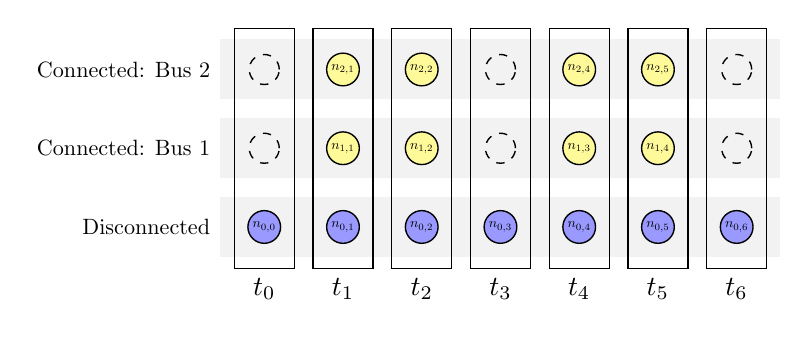
\begin{tikzpicture} 
			\node[rectangle, fill=gray!10, minimum width=2.8in, minimum height=.3in,label=left:\scalebox{0.8}{Connected: Bus 2}](bus2Box) at (3,1){};
			\node[rectangle, fill=gray!10, minimum width=2.8in, minimum height=.3in,label=left:\scalebox{0.8}{Connected: Bus 1}](bus1Box) at (3,0){};
			\node[rectangle, fill=gray!10, minimum width=2.8in, minimum height=.3in,label=left:\scalebox{0.8}{Disconnected}](bus1Box) at (3,-1){};

			\node[circle, draw, dashed,   line width=0.5pt, draw=black, minimum size=0.15in, inner sep=1pt](one)   at (0,0){};
			\node[circle, fill=yellow!40, line width=0.5pt, draw=black, minimum size=0.15in, inner sep=1pt](two)   at (1,0){\scalebox{0.5}{$n_{1,1}$}}; 
			\node[circle, fill=yellow!40, line width=0.5pt, draw=black, minimum size=0.15in, inner sep=1pt](three) at (2,0){\scalebox{0.5}{$n_{1,2}$}};
			\node[circle, draw, dashed,   line width=0.5pt, draw=black, minimum size=0.15in, inner sep=1pt](four)  at (3,0){};
			\node[circle, fill=yellow!40, line width=0.5pt, draw=black, minimum size=0.15in, inner sep=1pt](five)  at (4,0){\scalebox{0.5}{$n_{1,3}$}};
			\node[circle, fill=yellow!40, line width=0.5pt, draw=black, minimum size=0.15in, inner sep=1pt](six)   at (5,0){\scalebox{0.5}{$n_{1,4}$}};
			\node[circle, draw, dashed,   line width=0.5pt, draw=black, minimum size=0.15in, inner sep=1pt](seven) at (6,0){};

			\node[circle, draw, dashed,   line width=0.5pt, draw=black, minimum size=0.15in, inner sep=1pt](eight)    at (0,1){};
			\node[circle, fill=yellow!40, line width=0.5pt, draw=black, minimum size=0.15in, inner sep=1pt](nine)     at (1,1){\scalebox{0.5}{$n_{2,1}$}}; 
			\node[circle, fill=yellow!40, line width=0.5pt, draw=black, minimum size=0.15in, inner sep=1pt](ten)      at (2,1){\scalebox{0.5}{$n_{2,2}$}};
			\node[circle, draw, dashed,   line width=0.5pt, draw=black, minimum size=0.15in, inner sep=1pt](eleven)   at (3,1){};
			\node[circle, fill=yellow!40, line width=0.5pt, draw=black, minimum size=0.15in, inner sep=1pt](twelve)   at (4,1){\scalebox{0.5}{$n_{2,4}$}};
			\node[circle, fill=yellow!40, line width=0.5pt, draw=black, minimum size=0.15in, inner sep=1pt](thirteen) at (5,1){\scalebox{0.5}{$n_{2,5}$}};
			\node[circle, draw, dashed,   line width=0.5pt, draw=black, minimum size=0.15in, inner sep=1pt](fourteen) at (6,1){};

			\node[circle, fill=blue!40,   line width=0.5pt, draw=black, minimum size=0.15in, inner sep=1pt](eight)    at (0,-1){\scalebox{0.5}{$n_{0,0}$}};
			\node[circle, fill=blue!40,   line width=0.5pt, draw=black, minimum size=0.15in, inner sep=1pt](nine)     at (1,-1){\scalebox{0.5}{$n_{0,1}$}}; 
			\node[circle, fill=blue!40,   line width=0.5pt, draw=black, minimum size=0.15in, inner sep=1pt](ten)      at (2,-1){\scalebox{0.5}{$n_{0,2}$}};
			\node[circle, fill=blue!40,   line width=0.5pt, draw=black, minimum size=0.15in, inner sep=1pt](eleven)   at (3,-1){\scalebox{0.5}{$n_{0,3}$}};
			\node[circle, fill=blue!40,   line width=0.5pt, draw=black, minimum size=0.15in, inner sep=1pt](twelve)   at (4,-1){\scalebox{0.5}{$n_{0,4}$}};
			\node[circle, fill=blue!40,   line width=0.5pt, draw=black, minimum size=0.15in, inner sep=1pt](thirteen) at (5,-1){\scalebox{0.5}{$n_{0,5}$}};
			\node[circle, fill=blue!40,   line width=0.5pt, draw=black, minimum size=0.15in, inner sep=1pt](fourteen) at (6,-1){\scalebox{0.5}{$n_{0,6}$}};

			\node[rectangle, draw, minimum width=0.3in, minimum height=1.2in,label=below:$t_0$](time0Box) at (0,0){};
			\node[rectangle, draw, minimum width=0.3in, minimum height=1.2in,label=below:$t_1$](time1Box) at (1,0){};
			\node[rectangle, draw, minimum width=0.3in, minimum height=1.2in,label=below:$t_2$](time2Box) at (2,0){};
			\node[rectangle, draw, minimum width=0.3in, minimum height=1.2in,label=below:$t_3$](time3Box) at (3,0){};
			\node[rectangle, draw, minimum width=0.3in, minimum height=1.2in,label=below:$t_4$](time4Box) at (4,0){};
			\node[rectangle, draw, minimum width=0.3in, minimum height=1.2in,label=below:$t_5$](time5Box) at (5,0){};
			\node[rectangle, draw, minimum width=0.3in, minimum height=1.2in,label=below:$t_6$](time6Box) at (6,0){}; 
		\end{tikzpicture}
	}
		\caption{Bus availability represented in a graph}
		\label{fig:busAvailComparison}
\end{figure*}

\par Transitions from one node to the next are called edges (see figure \ref{fig:edgeNodeRel}) and represent decisions to either connect, charge, not charge, or disconnect. The decision an edge represents is determined by the nodes to either side. An edge which exits and enters no-charge nodes represents a period where chargers are disconnected, resulting in a no-charge decision. Similarly, edges which both enter and exit charge nodes indicate a to-charge decision. Both to-charge and no-charge decisions transitions represent \textit{horizontal} shifts in the graph and do not change the effective state of the charger. Conversely, transitions between no-charge and to-charge nodes represent effective state changes. A no-charge to charge connection is disconnected at $t_j$ and connected at $t_{j+1}$, indicating a decision to connect. The same logic applies for a disconnection where an edge begins connected and ends disconnected (see figure \ref{fig:edgeTypes}). Hence, the bus charge problem can be described in terms of nodes and edges where nodes represent in-station time periods and edges give all possible charge options as shown in figure \ref{fig:completeGraph}.
\par \textit{Making} decisions is encoded in the weight of each edge.  The value of each weight is used to represent the number of chargers in the transition. For example, if two chargers were left unused from $t_n$ to $t_{n+1}$, the corresponding edge would span two no-charge nodes, and have a weight value of two.

\begin{figure}
	\centering
	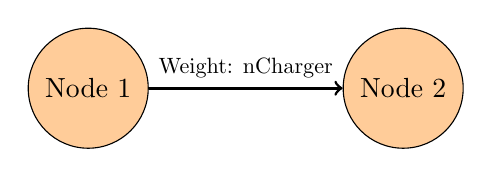
\begin{tikzpicture}
		\node[circle, draw, fill=orange!40, minimum size=0.6in](node1) at (0,0){Node 1};
		\node[circle, draw, fill=orange!40, minimum size=0.6in](node2) at (4,0){Node 2};
		\draw [->, line width=1pt] (node1.east) -- node[above]{\scalebox{0.8}{Weight: nCharger}}(node2.west); 
	\end{tikzpicture}
	\caption{Node to Node Connection}
	\label{fig:edgeNodeRel}
\end{figure}

\begin{figure}
	\centering
	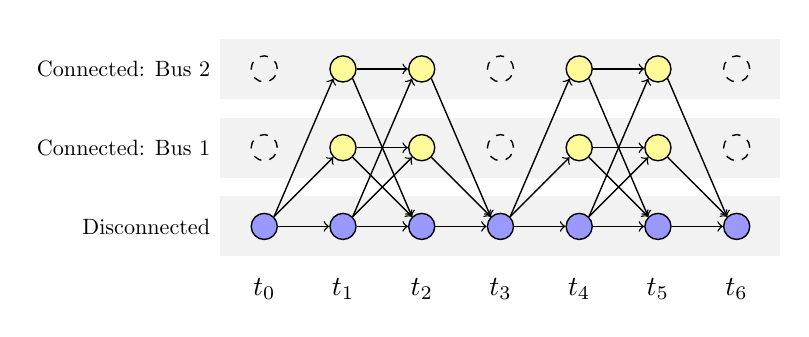
\begin{tikzpicture} 
		\node[rectangle, fill=gray!10, minimum width=2.8in, minimum height=.3in,label=left:\scalebox{0.8}{Connected: Bus 2}](bus2Box) at (3,1){};
		\node[rectangle, fill=gray!10, minimum width=2.8in, minimum height=.3in,label=left:\scalebox{0.8}{Connected: Bus 1}](bus1Box) at (3,0){};
		\node[rectangle, fill=gray!10, minimum width=2.8in, minimum height=.3in,label=left:\scalebox{0.8}{Disconnected}](bus1Box) at (3,-1){};

		\node[circle, draw, dashed, line width=0.5pt, draw=black, minimum size=0.1in](one) at (0,0){};
		\node[circle, fill=yellow!40, line width=0.5pt, draw=black, minimum size=0.1in](two) at (1,0){}; 
		\node[circle, fill=yellow!40, line width=0.5pt, draw=black, minimum size=0.1in](three) at (2,0){};
		\node[circle, draw, dashed, line width=0.5pt, draw=black, minimum size=0.1in](four) at (3,0){};
		\node[circle, fill=yellow!40, line width=0.5pt, draw=black, minimum size=0.1in](five) at (4,0){};
		\node[circle, fill=yellow!40, line width=0.5pt, draw=black, minimum size=0.1in](six) at (5,0){};
		\node[circle, draw, dashed,  line width=0.5pt, draw=black, minimum size=0.1in](seven) at (6,0){};

		\node[circle, draw, dashed, line width=0.5pt, draw=black, minimum size=0.1in](eight) at (0,1){};
		\node[circle, fill=yellow!40, line width=0.5pt, draw=black, minimum size=0.1in](nine) at (1,1){}; 
		\node[circle, fill=yellow!40, line width=0.5pt, draw=black, minimum size=0.1in](ten) at (2,1){};
		\node[circle, draw, dashed, line width=0.5pt, draw=black, minimum size=0.1in](eleven) at (3,1){};
		\node[circle, fill=yellow!40, line width=0.5pt, draw=black, minimum size=0.1in](twelve) at (4,1){};
		\node[circle, fill=yellow!40, line width=0.5pt, draw=black, minimum size=0.1in](thirteen) at (5,1){};
		\node[circle, draw, dashed, line width=0.5pt, draw=black, minimum size=0.1in](fourteen) at (6,1){};

		\node[circle, fill=blue!40, line width=0.5pt, draw=black, minimum size=0.1in](bOne) at (0,-1){};
		\node[circle, fill=blue!40, line width=0.5pt, draw=black, minimum size=0.1in](bTwo) at (1,-1){}; 
		\node[circle, fill=blue!40, line width=0.5pt, draw=black, minimum size=0.1in](bThree) at (2,-1){};
		\node[circle, fill=blue!40, line width=0.5pt, draw=black, minimum size=0.1in](bFour) at (3,-1){};
		\node[circle, fill=blue!40, line width=0.5pt, draw=black, minimum size=0.1in](bFive) at (4,-1){};
		\node[circle, fill=blue!40, line width=0.5pt, draw=black, minimum size=0.1in](bSix) at (5,-1){};
		\node[circle, fill=blue!40, line width=0.5pt, draw=black, minimum size=0.1in](bSeven) at (6,-1){};

		\node[rectangle, minimum width=0.3in, minimum height=1.2in,label=below:$t_0$](time0Box) at (0,0){};
		\node[rectangle, minimum width=0.3in, minimum height=1.2in,label=below:$t_1$](time1Box) at (1,0){};
		\node[rectangle, minimum width=0.3in, minimum height=1.2in,label=below:$t_2$](time2Box) at (2,0){};
		\node[rectangle, minimum width=0.3in, minimum height=1.2in,label=below:$t_3$](time3Box) at (3,0){};
		\node[rectangle, minimum width=0.3in, minimum height=1.2in,label=below:$t_4$](time4Box) at (4,0){};
		\node[rectangle, minimum width=0.3in, minimum height=1.2in,label=below:$t_5$](time5Box) at (5,0){};
		\node[rectangle, minimum width=0.3in, minimum height=1.2in,label=below:$t_6$](time6Box) at (6,0){}; 
		
		% draw rest edges
		\draw[->, line width=0.5pt] (bOne.east) -- (bTwo.west);
		\draw[->, line width=0.5pt] (bTwo.east) -- (bThree.west);
		\draw[->, line width=0.5pt] (bThree.east) -- (bFour.west);
		\draw[->, line width=0.5pt] (bFour.east) -- (bFive.west);
		\draw[->, line width=0.5pt] (bFive.east) -- (bSix.west);
		\draw[->, line width=0.5pt] (bSix.east) -- (bSeven.west);
		
		% draw connect edges
		\draw[->, line width=0.5pt] (bOne.north east) -- (two.south west); 
		\draw[->, line width=0.5pt] (bTwo.north east) -- (three.south west);
		\draw[->, line width=0.5pt] (bFour.north east) -- (five.south west);
		\draw[->, line width=0.5pt] (bFive.north east) -- (six.south west);

		\draw[->, line width=0.5pt] (bOne.north east) -- (nine.south west);
		\draw[->, line width=0.5pt] (bTwo.north east) -- (ten.south west);
		\draw[->, line width=0.5pt] (bFour.north east) -- (twelve.south west);
		\draw[->, line width=0.5pt] (bFive.north east) -- (thirteen.south west);

		% draw disconnect edges
		\draw[->, line width=0.5pt] (two.south east) -- (bThree.north west); 
		\draw[->, line width=0.5pt] (three.south east) -- (bFour.north west);
		\draw[->, line width=0.5pt] (five.south east) -- (bSix.north west);
		\draw[->, line width=0.5pt] (six.south east) -- (bSeven.north west);

		\draw[->, line width=0.5pt] (nine.south east) -- (bThree.north west);
		\draw[->, line width=0.5pt] (ten.south east) -- (bFour.north west);
		\draw[->, line width=0.5pt] (twelve.south east) -- (bSix.north west);
		\draw[->, line width=0.5pt] (thirteen.south east) -- (bSeven.north west);

		% draw charge edges
		\draw[->, line width=0.5pt] (two.east) -- (three.west);
		\draw[->, line width=0.5pt] (five.east) -- (six.west);
		\draw[->, line width=0.5pt] (nine.east) -- (ten.west);
		\draw[->, line width=0.5pt] (twelve.east) -- (thirteen.west);

	\end{tikzpicture}
	\caption{Complete Problem formulation}
	\label{fig:completeGraph}
\end{figure}
\begin{figure}
	\centering
	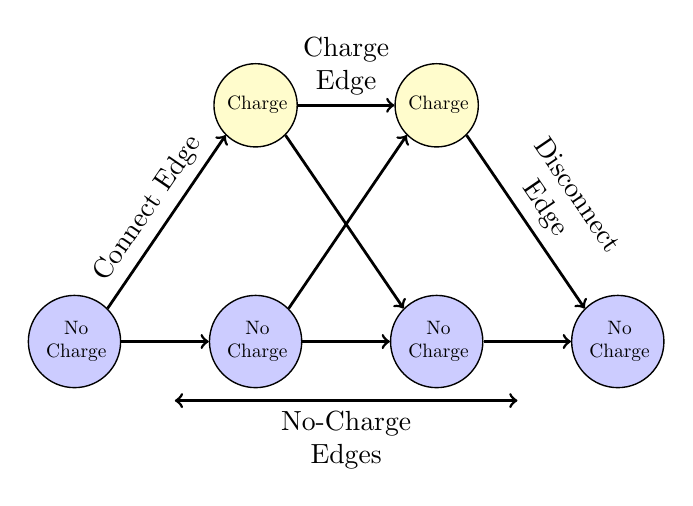
\begin{tikzpicture}
		\node[circle, fill=blue!20,line width=0.5pt, draw=black, text width=0.4in, inner sep=0in](one) at (0,0){\scalebox{0.7}{\begin{tabular}{c}No\\ Charge \end{tabular}}};
		\node[circle, fill=blue!20,line width=0.5pt, draw=black, text width=0.4in, inner sep=0in](two) at (2.3,0){\scalebox{0.7}{\begin{tabular}{c}No\\ Charge \end{tabular}}};
		\node[circle, fill=blue!20,line width=0.5pt, draw=black, text width=0.4in, inner sep=0in](three) at (4.6,0){\scalebox{0.7}{\begin{tabular}{c}No\\ Charge \end{tabular}}};
		\node[circle, fill=blue!20,line width=0.5pt, draw=black, text width=0.4in, inner sep=0in](four) at (6.9,0){\scalebox{0.7}{\begin{tabular}{c}No\\ Charge \end{tabular}}};
		\node[circle, fill=yellow!20,line width=0.5pt, draw=black, text width=0.4in, inner sep=0in](five) at (2.3,3){\scalebox{0.7}{\begin{tabular}{c} Charge \end{tabular}}};
		\node[circle, fill=yellow!20,line width=0.5pt, draw=black, text width=0.4in, inner sep=0in](six) at (4.6,3){\scalebox{0.7}{\begin{tabular}{c}Charge \end{tabular}}};
		\node(placeholder1) at (1.15,-0.75){};
		\node(placeholder2) at (5.75,-0.75){};
		\draw [->, line width=1pt] (one.north east) -- node[sloped, anchor=center, above, text width=2.5cm, midway, align=center]{Connect Edge}(five.south west);
		\draw [->, line width=1pt] (one.east) -- (two.west);
		\draw [->, line width=1pt] (five.east) -- node[sloped, anchor=center, above, text width=1.5cm, midway, align=center]{Charge Edge}(six.west);
		\draw [->, line width=1pt] (five.south east) -- (three.north west);
		\draw [->, line width=1pt] (two.north east) -- (six.south west);
		\draw [->, line width=1pt] (six.south east) -- node[sloped, anchor=center, above, text width=1.5cm, midway, align=center]{Disconnect Edge}(four.north west);
		\draw [->, line width=1pt] (two.east) -- (three.west);
		\draw [->, line width=1pt] (three.east) -- (four.west); 
		\draw [<->, line width=1pt] (placeholder1) -- node[below, text width=2cm, midway, align=center]{No-Charge Edges}(placeholder2);
	\end{tikzpicture}
	\caption{Connect, Disconnect, and Charge Edges}
	\label{fig:edgeTypes}
\end{figure}


\par Consider a two-charger scenario where buses follow the schedule given in figure \ref{fig:completeGraph}. A solution where Bus 1 charges from $t_1$ to $t_2$ and Bus 2 charges from $t_4$ to $t_5$ would be expressed by assigning non-zero weights to the appropriate connect, charge, and disconnect edges as shown in figure \ref{fig:graphWithSolution}.  Thus, solving the bus charge problem becomes a matter of finding the optimal set of edge weights.

\begin{figure}
	\centering
	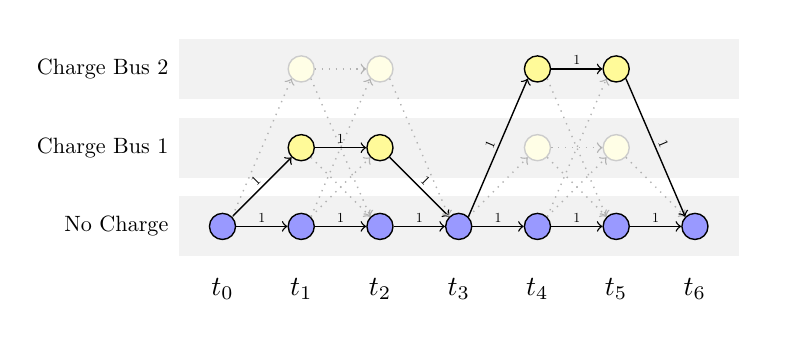
\begin{tikzpicture} 
		\node[rectangle, fill=gray!10, minimum width=2.8in, minimum height=.3in,label=left:\scalebox{0.8}{Charge Bus 2}](bus2Box) at (3,1){};
		\node[rectangle, fill=gray!10, minimum width=2.8in, minimum height=.3in,label=left:\scalebox{0.8}{Charge Bus 1}](bus1Box) at (3,0){};
		\node[rectangle, fill=gray!10, minimum width=2.8in, minimum height=.3in,label=left:\scalebox{0.8}{No Charge}](bus1Box) at (3,-1){};

		\node[circle, fill=yellow!40, line width=0.5pt, draw=black, minimum size=0.1in](two) at (1,0){}; 
		\node[circle, fill=yellow!40, line width=0.5pt, draw=black, minimum size=0.1in](three) at (2,0){};
		\node[circle, fill=yellow!10, line width=0.5pt, draw=black!20, minimum size=0.1in](five) at (4,0){};
		\node[circle, fill=yellow!10, line width=0.5pt, draw=black!20, minimum size=0.1in](six) at (5,0){};

		\node[circle, fill=yellow!10, line width=0.5pt, draw=black!20, minimum size=0.1in](nine) at (1,1){}; 
		\node[circle, fill=yellow!10, line width=0.5pt, draw=black!20, minimum size=0.1in](ten) at (2,1){};
		\node[circle, fill=yellow!40, line width=0.5pt, draw=black, minimum size=0.1in](twelve) at (4,1){};
		\node[circle, fill=yellow!40, line width=0.5pt, draw=black, minimum size=0.1in](thirteen) at (5,1){};

		\node[circle, fill=blue!40, line width=0.5pt, draw=black, minimum size=0.1in](bOne) at (0,-1){};
		\node[circle, fill=blue!40, line width=0.5pt, draw=black, minimum size=0.1in](bTwo) at (1,-1){}; 
		\node[circle, fill=blue!40, line width=0.5pt, draw=black, minimum size=0.1in](bThree) at (2,-1){};
		\node[circle, fill=blue!40, line width=0.5pt, draw=black, minimum size=0.1in](bFour) at (3,-1){};
		\node[circle, fill=blue!40, line width=0.5pt, draw=black, minimum size=0.1in](bFive) at (4,-1){};
		\node[circle, fill=blue!40, line width=0.5pt, draw=black, minimum size=0.1in](bSix) at (5,-1){};
		\node[circle, fill=blue!40, line width=0.5pt, draw=black, minimum size=0.1in](bSeven) at (6,-1){};

		\node[rectangle, minimum width=0.3in, minimum height=1.2in,label=below:$t_0$](time0Box) at (0,0){};
		\node[rectangle, minimum width=0.3in, minimum height=1.2in,label=below:$t_1$](time1Box) at (1,0){};
		\node[rectangle, minimum width=0.3in, minimum height=1.2in,label=below:$t_2$](time2Box) at (2,0){};
		\node[rectangle, minimum width=0.3in, minimum height=1.2in,label=below:$t_3$](time3Box) at (3,0){};
		\node[rectangle, minimum width=0.3in, minimum height=1.2in,label=below:$t_4$](time4Box) at (4,0){};
		\node[rectangle, minimum width=0.3in, minimum height=1.2in,label=below:$t_5$](time5Box) at (5,0){};
		\node[rectangle, minimum width=0.3in, minimum height=1.2in,label=below:$t_6$](time6Box) at (6,0){}; 
		
		% draw rest edges
		\draw[->, line width=0.5pt] (bOne.east) -- node [text width=2.5cm, midway, above=-2.1pt, align=center]{\scalebox{0.5}{1}}(bTwo.west);
		\draw[->, line width=0.5pt] (bTwo.east) -- node [text width=2.5cm, midway, above=-2.1pt, align=center]{\scalebox{0.5}{1}}(bThree.west);
		\draw[->, line width=0.5pt] (bThree.east) -- node [text width=2.5cm, midway, above=-2.1pt, align=center]{\scalebox{0.5}{1}}(bFour.west);
		\draw[->, line width=0.5pt] (bFour.east) -- node [text width=2.5cm, midway, above=-2.1pt, align=center]{\scalebox{0.5}{1}}(bFive.west);
		\draw[->, line width=0.5pt] (bFive.east) -- node [text width=2.5cm, midway, above=-2.1pt, align=center]{\scalebox{0.5}{1}}(bSix.west);
		\draw[->, line width=0.5pt] (bSix.east) -- node [text width=2.5cm, midway, above=-2.1pt, align=center]{\scalebox{0.5}{1}}(bSeven.west);
		
		% draw connect edges
		\draw[->, line width=0.5pt] (bOne.north east) -- node [sloped, text width=2.5cm, midway, above=-2.1pt, align=center]{\scalebox{0.5}{1}}(two.south west); 
		\draw[->, dotted, color=black!30, line width=0.5pt] (bTwo.north east) -- (three.south west);
		\draw[->, dotted, color=black!30, line width=0.5pt] (bFour.north east) -- (five.south west);
		\draw[->, dotted, color=black!30, line width=0.5pt] (bFive.north east) -- (six.south west);

		\draw[->, dotted, color=black!30, line width=0.5pt] (bOne.north east) -- (nine.south west);
		\draw[->, dotted, color=black!30, line width=0.5pt] (bTwo.north east) -- (ten.south west);
		\draw[->, line width=0.5pt] (bFour.north east) -- node [sloped, text width=2.5cm, midway, above=-2.1pt, align=center]{\scalebox{0.5}{1}}(twelve.south west);
		\draw[->, dotted, color=black!30, line width=0.5pt] (bFive.north east) -- (thirteen.south west);

		% draw disconnect edges
		\draw[->, dotted, color=black!30, line width=0.5pt] (two.south east) -- (bThree.north west); 
		\draw[->, line width=0.5pt] (three.south east) -- node [sloped, text width=2.5cm, midway, above=-2.1pt, align=center]{\scalebox{0.5}{1}}(bFour.north west);
		\draw[->, dotted, color=black!30, line width=0.5pt] (five.south east) -- (bSix.north west);
		\draw[->, dotted, color=black!30, line width=0.5pt] (six.south east) -- (bSeven.north west);

		\draw[->, dotted, color=black!30, line width=0.5pt] (nine.south east) -- (bThree.north west);
		\draw[->, dotted, color=black!30, line width=0.5pt] (ten.south east) -- (bFour.north west);
		\draw[->, dotted, color=black!30, line width=0.5pt] (twelve.south east) -- (bSix.north west);
		\draw[->, line width=0.5pt] (thirteen.south east) -- node [sloped, text width=2.5cm, midway, above=-2.1pt, align=center]{\scalebox{0.5}{1}}(bSeven.north west);

		% draw charge edges
		\draw[->, line width=0.5pt] (two.east) -- node [text width=2.5cm, midway, above=-2.1pt, align=center]{\scalebox{0.5}{1}}(three.west);
		\draw[->, dotted, color=black!30, line width=0.5pt] (five.east) -- (six.west);
		\draw[->, dotted, color=black!30, line width=0.5pt] (nine.east) -- (ten.west);
		\draw[->, line width=0.5pt] (twelve.east) -- node [text width=2.5cm, midway, above=-2.1pt, align=center]{\scalebox{0.5}{1}}(thirteen.west); 
	\end{tikzpicture}
	\caption{One solution to a 2-bus 2-charger scenario}
	\label{fig:graphWithSolution}
\end{figure}



\par To find the optimal set of weights, the graph must first be encoded in an incidence matrix. An incidence matrix organizes relationships between nodes and edges by describing which edges depart from and connect to which nodes. An incidence matrix $A$ is an nNode $\times$ nEdge matrix where nNode is the number of nodes, and nEdge is the number of edges. 
\par The columns of $A$ describe connections for each edge and the rows give connections for each node. Incoming connections are represented with $1$, outgoing connections with $-1$, and no connection with $0$. For example, the graph in figure \ref{fig:genericGraph} is represented as:
\begin{figure}
	\centering
	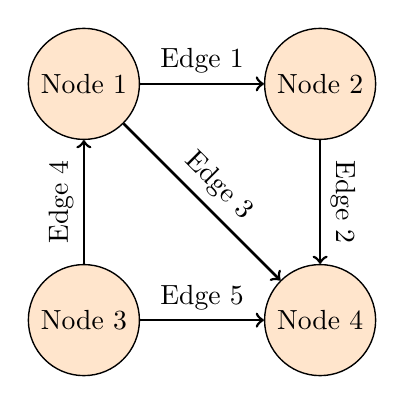
\begin{tikzpicture}
		\node[circle, line width=0.5pt, draw=black, fill=orange!20, minimum size=0.5in](topLeft) at (0,3){Node 1};
		\node[circle, line width=0.5pt, draw=black, fill=orange!20, minimum size=0.5in](topRight) at (3,3){Node 2};
		\node[circle, line width=0.5pt, draw=black, fill=orange!20, minimum size=0.5in](btmLeft) at (0,0){Node 3};
		\node[circle, line width=0.5pt, draw=black, fill=orange!20, minimum size=0.5in](btmRight) at (3,0){Node 4};
		\draw [->, line width=1pt] (topLeft.east) -- node [text width=2.5cm, midway, above, align=center]{Edge 1}(topRight.west);
		\draw [->, line width=1pt] (btmLeft.north) -- node [sloped, anchor=center, above, text width=2.5cm, midway, align=center]{Edge 4}(topLeft.south);
		\draw [->, line width=1pt] (topLeft.south east) -- node [sloped, anchor=center, above, text width=2.5cm, midway, align=center]{Edge 3}(btmRight.north west);
		\draw [->, line width=1pt] (topRight.south) -- node[sloped, anchor=center, above, text width=2.5cm, midway, align=center]{Edge 2}(btmRight.north);
		\draw [->, line width=1pt] (btmLeft.east) -- node[text width=2.5cm, midway, above, align=center]{Edge 5}(btmRight.west);
	\end{tikzpicture}
	\caption{A generic directed graph consisting of nodes and edges}
	\label{fig:genericGraph}
\end{figure}
\begin{align}
	\begin{bmatrix}
		-1 & 0 & -1 & 1 & 0 \\
		1 & -1 & 0 & 0 & 0 \\
		0 & 0 & 0 & -1 & -1 \\
		0 & 1 & 1 & 0 & 1 \\
	\end{bmatrix}
\end{align}
\par  An incidence matrix can be used to find the number of chargers entering and leaving each state. None of the states (charging/non-charging) can create or destroy chargers and so the number of incoming must always equal the number of outgoing chargers. The only exception occurs at \textit{source} and \textit{sink} nodes.
\par A source node represents the beginning state of all chargers.  Because a source state is the first, there are no incoming edges and hence, the net difference between incoming and outgoing chargers, or \textit{the net-flow}, will be minus the number of chargers. 
\par Sink nodes represent the final state, where all chargers enter and finish (see figure \ref{fig:sourceSink}). Because sinks have no outgoing edges, they maintain a positive net-flow equal to the number of chargers. 
\par Let $x$ be a vector representing the edge weights, $A$ be an adjacency matrix, and $c_f$ be a vector where $c_{f_i}$ gives the net-flow for the $i^{\text{th}}$ node. The net-flow for each node can be expressed as 

\begin{figure}
	\centering
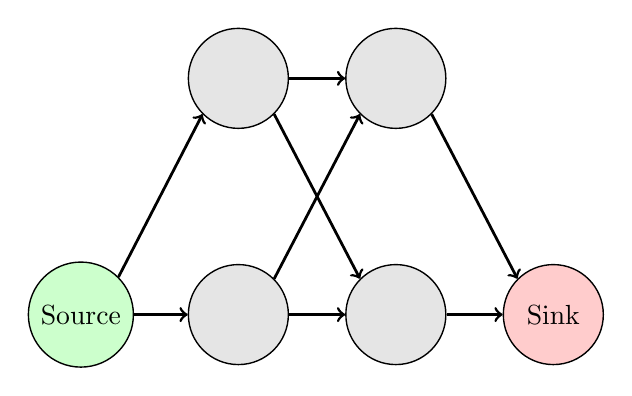
\begin{tikzpicture}
	\node[circle, fill=green!20, line width=0.5pt, draw=black, minimum size=0.5in](one) at (0,0){Source};
	\node[circle, fill=gray!20,line width=0.5pt, draw=black, minimum size=0.5in](two) at (2,0){};
	\node[circle, fill=gray!20,line width=0.5pt, draw=black, minimum size=0.5in](three) at (4,0){};
	\node[circle, fill=red!20,line width=0.5pt, draw=black, minimum size=0.5in](four) at (6,0){Sink};
	\node[circle, fill=gray!20, line width=0.5pt, draw=black, minimum size=0.5in](five) at (2,3){};
	\node[circle, fill=gray!20, line width=0.5pt, draw=black, minimum size=0.5in](six) at (4,3){};
	\draw [->, line width=1pt] (one.north east) -- (five.south west);
	\draw [->, line width=1pt] (one.east) -- (two.west);
	\draw [->, line width=1pt] (five.east) -- (six.west);
	\draw [->, line width=1pt] (five.south east) -- (three.north west);
	\draw [->, line width=1pt] (two.north east) -- (six.south west);
	\draw [->, line width=1pt] (six.south east) -- (four.north west);
	\draw [->, line width=1pt] (two.east) -- (three.west);
	\draw [->, line width=1pt] (three.east) -- (four.west); 
\end{tikzpicture}
	\caption{Network flow illustrating sources and sinks}
	\label{fig:sourceSink} 
\end{figure} 

\begin{align}
	Ax = c_f
\end{align}
This expression can be used to constrain the net-flow of each node.  $c_f$ must equal zero for all non-source and non-sink elements and source/sink nodes must have net-flows equal to $-\text{nChargers}$ and nChargers respectively (see equation \ref{eqn:cFlow}).
\begin{align}\label{eqn:cFlow}
	Ax = \begin{bmatrix} 0 \\ \vdots \\ -\text{nCharger} \\ \vdots \\ 0 \\ \text{nCharger} \\ \vdots \\ 0\end{bmatrix}
\end{align}

\par Flow can also be used to ensure that buses connect to only one charger at a time. Let a charge session, or \textit{group}, be the set of all charge nodes between routes as shown in figure \ref{fig:groups}. The \textit{group flow} is the number of chargers that enter a group and is represented as the sum of all incoming edge weights (see figure \ref{fig:groupedEdges}). 
\par Let $B$ be a nGroup $\times$ nEdge matrix where $B_{i,j}$ is $1$ if the $j^{\text{th}}$ edge enters the $i^{\text{th}}$ group and $0$ otherwise. For example, the $B$ matrix corresponding to the graph in figure \ref{fig:groupEdges} contains $1$ in the $7^{\text{th}}$ and $10^{\text{th}}$ columns for Group 1, and the $12^{\text{th}}$ and $15^{\text{th}}$ columns for group 2 as given in equation \ref{eqn:groupB}.
\begin{align}\label{eqn:groupB}
	B = \begin{bmatrix}0 \; 0 \; 0 \; 0 \; 0 \; 0 \; 1 \; 0 \; 0 \; 1 \; 0 \; 0 \; 0 \; 0 \; 0 \; 0\\
	                   0 \; 0 \; 0 \; 0 \; 0 \; 0 \; 0 \; 0 \; 0 \; 0 \; 0 \; 1 \; 0 \; 0 \; 1 \; 0\end{bmatrix}
\end{align}

\begin{figure}
	\centering
	\begin{tikzpicture}
		\node[circle, fill=blue!20, line width=0.5pt, draw=black, minimum size=0.1in](one) at (0,0){};
		\node[circle, fill=blue!20, line width=0.5pt, draw=black, minimum size=0.1in](two) at (1,0){}; 
		\node[circle, fill=blue!20, line width=0.5pt, draw=black, minimum size=0.1in](three) at (2,0){};
		\node[circle, fill=blue!20, line width=0.5pt, draw=black, minimum size=0.1in](four) at (3,0){};
		\node[circle, fill=blue!20, line width=0.5pt, draw=black, minimum size=0.1in](five) at (4,0){};
		\node[circle, fill=blue!20, line width=0.5pt, draw=black, minimum size=0.1in](six) at (5,0){};
		\node[circle, fill=blue!20, line width=0.5pt, draw=black, minimum size=0.1in](seven) at (6,0){};
		\node[circle, fill=yellow!20, line width=0.5pt, draw=black, minimum size=0.1in](eight) at (1,2){};
		\node[circle, fill=yellow!20, line width=0.5pt, draw=black, minimum size=0.1in](nine) at (2,2){};
		\node[circle, fill=yellow!20, line width=0.5pt, draw=black, minimum size=0.1in](ten) at (4,2){}; 
		\node[circle, fill=yellow!20, line width=0.5pt, draw=black, minimum size=0.1in](eleven) at (5,2){}; 
		\draw [->, line width=0.5pt] (one.east) -- (two.west);
		\draw [->, line width=0.5pt] (two.east) -- (three.west);
		\draw [->, line width=0.5pt] (three.east) -- (four.west);
		\draw [->, line width=0.5pt] (four.east) -- (five.west);
		\draw [->, line width=0.5pt] (five.east) -- (six.west);
		\draw [->, line width=0.5pt] (six.east) -- (seven.west);
		\draw [->, line width=0.5pt] (one.north east) -- (eight.south west);
		\draw [->, line width=0.5pt] (two.north east) -- (nine.south west);
		\draw [->, line width=0.5pt] (four.north east) -- (ten.south west);
		\draw [->, line width=0.5pt] (five.north east) -- (eleven.south west);
		\draw [->, line width=0.5pt] (eight.south east) -- (three.north west);
		\draw [->, line width=0.5pt] (nine.south east) -- (four.north west);
		\draw [->, line width=0.5pt] (ten.south east) -- (six.north west);
		\draw [->, line width=0.5pt] (eleven.south east) -- (seven.north west);
		\draw [->, line width=0.5pt] (eight.east) -- (nine.west);
		\draw [->, line width=0.5pt] (ten.east) -- (eleven.west); 
		\node[ellipse, fill opacity=0.2, draw opacity=0.5, line width=0.5pt, draw=orange!40,fill=orange!40, minimum height=0.4in, minimum width=1in, label=Group 1](group1) at (1.5,2){};
		\node[ellipse, fill opacity=0.2, draw opacity=0.5, line width=0.5pt, draw=purple!40,fill=purple!40,  minimum height=0.4in, minimum width=1in, label=Group 2](group2) at (4.5,2){};
	\end{tikzpicture}
	\caption{Example of groups in a network flow graph}
	\label{fig:groups}
\end{figure}
\begin{figure}
\centering
	\begin{tikzpicture}
		\node[circle, fill=blue!20, line width=0.5pt, draw=black, minimum size=0.1in](one) at (0,0){};
		\node[circle, fill=blue!20, line width=0.5pt, draw=black, minimum size=0.1in](two) at (1,0){}; 
		\node[circle, fill=blue!20, line width=0.5pt, draw=black, minimum size=0.1in](three) at (2,0){};
		\node[circle, fill=blue!20, line width=0.5pt, draw=black, minimum size=0.1in](four) at (3,0){};
		\node[circle, fill=blue!20, line width=0.5pt, draw=black, minimum size=0.1in](five) at (4,0){};
		\node[circle, fill=blue!20, line width=0.5pt, draw=black, minimum size=0.1in](six) at (5,0){};
		\node[circle, fill=blue!20, line width=0.5pt, draw=black, minimum size=0.1in](seven) at (6,0){};
		\node[circle, fill=yellow!20, line width=0.5pt, draw=black, minimum size=0.1in](eight) at (1,2){};
		\node[circle, fill=yellow!20, line width=0.5pt, draw=black, minimum size=0.1in](nine) at (2,2){};
		\node[circle, fill=yellow!20, line width=0.5pt, draw=black, minimum size=0.1in](ten) at (4,2){}; 
		\node[circle, fill=yellow!20, line width=0.5pt, draw=black, minimum size=0.1in](eleven) at (5,2){}; 
		\draw [->, line width=0.5pt,color=black!40] (one.east) -- (two.west);
		\draw [->, line width=0.5pt,color=black!40] (two.east) -- (three.west);
		\draw [->, line width=0.5pt,color=black!40] (three.east) -- (four.west);
		\draw [->, line width=0.5pt,color=black!40] (four.east) -- (five.west);
		\draw [->, line width=0.5pt,color=black!40] (five.east) -- (six.west);
		\draw [->, line width=0.5pt,color=black!40] (six.east) -- (seven.west);
		\draw [->, color=orange, line width=0.75pt] (one.north east) -- (eight.south west);
		\draw [->, color=orange, line width=0.75pt] (two.north east) -- (nine.south west);
		\draw [->, color=purple, line width=0.75pt] (four.north east) -- (ten.south west);
		\draw [->, color=purple, line width=0.75pt] (five.north east) -- (eleven.south west);
		\draw [->, line width=0.5pt,color=black!40] (eight.south east) -- (three.north west);
		\draw [->, line width=0.5pt,color=black!40] (nine.south east) -- (four.north west);
		\draw [->, line width=0.5pt,color=black!40] (ten.south east) -- (six.north west);
		\draw [->, line width=0.5pt,color=black!40] (eleven.south east) -- (seven.north west);
		\draw [->, line width=0.5pt,color=black!40] (eight.east) -- (nine.west);
		\draw [->, line width=0.5pt,color=black!40] (ten.east) -- (eleven.west); 
		\node[ellipse, line width=0pt, draw opacity=0.5, fill opacity=0.2, fill=purple!40, draw=purple!40, minimum height=0.4in, minimum width=1in, label=Group 2](group2) at (4.5,2){};
		\node[ellipse, line width=0pt, draw opacity=0.5, fill opacity=0.2, fill=orange!40, draw=orange!40, minimum height=0.4in, minimum width=1in, label=Group 1](group1) at (1.5,2){};
	\end{tikzpicture}
	\caption{Incoming Group Edges}
	\label{fig:groupedEdges} 
\end{figure} 
Let $x$ be the edge weights as before and $c_g$ be an nGroup $\times$ 1 vector where the $i^{\text{th}}$ element gives the group flow for group $i$. The group flow is then computed as 
\begin{align}
	Bx = c_g
\end{align}
But the group flow is required to be one at most.  This is expressed by the inequality given in equation \ref{eqn:cGroupFlow}.
\begin{align}\label{eqn:cGroupFlow}
	Bx \le \begin{bmatrix} 1\\ 1 \\\vdots \\ 1\end{bmatrix},
\end{align}

\begin{figure}
\centering
	\begin{tikzpicture}
		\node[circle, fill=blue!20, line width=0.5pt, draw=black, minimum size=0.1in](one) at (0,0){};
		\node[circle, fill=blue!20, line width=0.5pt, draw=black, minimum size=0.1in](two) at (1,0){}; 
		\node[circle, fill=blue!20, line width=0.5pt, draw=black, minimum size=0.1in](three) at (2,0){};
		\node[circle, fill=blue!20, line width=0.5pt, draw=black, minimum size=0.1in](four) at (3,0){};
		\node[circle, fill=blue!20, line width=0.5pt, draw=black, minimum size=0.1in](five) at (4,0){};
		\node[circle, fill=blue!20, line width=0.5pt, draw=black, minimum size=0.1in](six) at (5,0){};
		\node[circle, fill=blue!20, line width=0.5pt, draw=black, minimum size=0.1in](seven) at (6,0){};
		\node[circle, fill=yellow!20, line width=0.5pt, draw=black, minimum size=0.1in](eight) at (1,2){};
		\node[circle, fill=yellow!20, line width=0.5pt, draw=black, minimum size=0.1in](nine) at (2,2){};
		\node[circle, fill=yellow!20, line width=0.5pt, draw=black, minimum size=0.1in](ten) at (4,2){}; 
		\node[circle, fill=yellow!20, line width=0.5pt, draw=black, minimum size=0.1in](eleven) at (5,2){}; 
		\node[ellipse, line width=0pt, draw=white, minimum height=0.4in, minimum width=1in, label=Group 1](group1) at (1.5,2){};
		\node[ellipse, line width=0pt, draw=white, minimum height=0.4in, minimum width=1in, label=Group 2](group2) at (4.5,2){};
		\draw [->, line width=0.5pt,color=black!40] (one.east) -- (two.west);
		\draw [->, line width=0.5pt,color=black!40] (two.east) -- (three.west);
		\draw [->, line width=0.5pt,color=black!40] (three.east) -- (four.west);
		\draw [->, line width=0.5pt,color=black!40] (four.east) -- (five.west);
		\draw [->, line width=0.5pt,color=black!40] (five.east) -- (six.west);
		\draw [->, line width=0.5pt,color=black!40] (six.east) -- (seven.west);
		\draw [->, color=orange, line width=0.75pt] (one.north east) -- node[sloped, anchor=center, above, text width=2.5cm, align=center]{Edge 7}(eight.south west);
		\draw [->, color=orange, line width=0.75pt] (two.north east) -- node[sloped, anchor=center, above, text width=2.5cm, align=center]{Edge 10}(nine.south west);
		\draw [->, color=purple, line width=0.75pt] (four.north east) -- node[sloped, anchor=center, above, text width=2.5cm, align=center]{Edge 12}(ten.south west);
		\draw [->, color=purple, line width=0.75pt] (five.north east) -- node[sloped, anchor=center, above, text width=2.5cm, align=center]{Edge 15}(eleven.south west);
		\draw [->, line width=0.5pt,color=black!40] (eight.south east) -- (three.north west);
		\draw [->, line width=0.5pt,color=black!40] (nine.south east) -- (four.north west);
		\draw [->, line width=0.5pt,color=black!40] (ten.south east) -- (six.north west);
		\draw [->, line width=0.5pt,color=black!40] (eleven.south east) -- (seven.north west);
		\draw [->, line width=0.5pt,color=black!40] (eight.east) -- (nine.west);
		\draw [->, line width=0.5pt,color=black!40] (ten.east) -- (eleven.west); 
	\end{tikzpicture}
	\caption{Connect edge example for groups}
	\label{fig:groupEdges} 
\end{figure} 
